\documentclass{article}

\usepackage[utf8]{inputenc}
% \usepackage[spanish, mexico]{babel}
\usepackage{blindtext}
\usepackage{graphicx}
\usepackage[pass]{geometry}
\usepackage[backend=bibtex]{biblatex}
\usepackage{float}
\usepackage{amsfonts}
\usepackage{parskip}

\addbibresource{bibliography.bib} %Imports bibliography file

\begin{document}

\newgeometry{bottom=2.8cm, left=2.8cm,right=2.8cm,top=2.8cm}

\title{Advanced operating Systems \\ Final project}

\author{Mario~Becerra Contreras \\ Luis Daniel~Hernández}

\date{Fall 2017}


\maketitle

\section{Introduction}

In this document, we present the implementation of a program that simulates a system to schedule I/O tasks, based on the \citeyear{mogul1997eliminating} paper \citetitle{mogul1997eliminating} by \citeauthor{mogul1997eliminating} \cite{mogul1997eliminating}. The document is organized as follows: first we present an overview of the original paper, then we explain the architecture and implementation strategy, we follow by showing the results, and finally we end with conclusions and lessons from this work.


\section{Methodology}

This section describes the system architecture and the theory behind it.

\subsection{Overview of \citetitle{mogul1997eliminating}}

At the time of the writing (\citeyear{mogul1997eliminating}), most OSs used interrupt systems to schedule I/O tasks. Polling could be used as an alternative to interrupts, but it was seldom used because of the increased latency of responses and excessive overhead. The drawbacks of interrupt systems are that they perform badly under overload and lead to a \textit{receive livelock}, where the system does not make progress on its tasks. In the paper, \citeauthor{mogul1997eliminating} presented modifications to an interrupt-driven system in order to achieve better performance using polling when the livelock condition is triggered, focusing on high throughput and low latency, as well as avoiding under-performance in other applications.

They defined an interrupt-driven system as follows: when a packet arrives, the CPU is interrupted and preempt all tasks with a lower priority. The packet is placed on a queue and causes a software interrupt so that packet can be further processed. The software interrupt is changed to a lower priority, which means that the processing of the packet can be preempted by subsequent interrupts. So, under a lot of interrupts, the throughput drops to zero and the system gets livelocked. Because of the design of most network adapters at the time, the rationale of giving absolute priority to the first few steps of packet reception was debunked.

Three main problems arise in interrupt-driven systems under heavy network input load: 1) receive livelock; 2) increased latency for delivery or forwarding because of the delay in delivery caused by the interrupts; and 3) starvation of packet transmission caused by the default lower priority of transmission in contrast to reception, which in an overloaded system leads to packets awaiting for transmission but the transmission interface is idle.

The techniques the authors proposed to avoid receive livelocks were:

\begin{itemize}
	\item \textbf{Limiting the interrupt arrival rate}: If the rate in which interrupts are imposed on the system is limited, then livelock can be avoided. When a system is about to drop a packet because a queue is full, then input interrupts should be disabled, and be re-enabled when buffer space is available.

	\item \textbf{Use of polling}: Since it's undesirable to have a poll-only system, then polling may be mixed with interrupts. During low loads, interrupts are used because packet arrivals are unpredictable; and during high loads, polling is used because one knows that packets are coming continuously. Interrupts are re-enabled when no more work is pending.

	\item \textbf{Avoiding preemption}: Livelocks occur because interrupts preempt other packet processing. This can be avoided by stopping the preemption of high-level packet processing.

\end{itemize}

They tested these techniques on an IP packet router, measuring router performance by counting the number of packets that were successfully forwarded in a given period. They compared an unmodified system against two modifications: one in which a maximum quota on packets processed for the same interface is used, and one with no quota. The result is that with no quotas, the performance is worse than on the unmodified system, but the quotas seem to have a much better performance and reach hardware limits. Then they compared performance based on different amounts of quota and see that quota of between 10 and 20 packets yields near-optimum behavior for the hardware they used.

The final issue that they tested was that with the modifications they made, packet processing was successful under overload, but this ignored the fact that user-level processed could be starving. The problem could be improved by measuring how much CPU time is spent in handling received packets and disabling the input when it's above a certain threshold, this threshold being a fraction of the total number of cycles in a period. They found that they could achieve stable behavior with high input rates.

\subsection{Architecture}

The system was implemented in Java, simulating $k$ I/O devices that are sent to $k$ receiver nodes, in a one-to-one mapping. The architecture can be seen in figure \ref{fig:arch_diagram}, where one can see that each one of the $k$ sending devices (each represented by a rectangle) is implemented with two threads, one for sending the message and one that is continuously listening and waiting for a signal to start polling. The sending threads (dashed lines) send a message to a middleware server queue which sends these messages to a receiver (represented by circles). The queue has a quota which that if is exceeded, the polling system replaces the interrupt system. The polling system uses a round-robin approach: it first asks client number 1 to send the packets the have and the resend it to the corresponding receiver, then it asks client number 2, and so on. The pure polling system can be used by setting the queue size to one, that way it overflows since the first message arrives and starts polling the receivers. After there is space in the queue again, the interrupt system is used again. In figure \ref{fig:uml_diagram} the UML of the system is shown.



\begin{figure}[H]
    \centering
    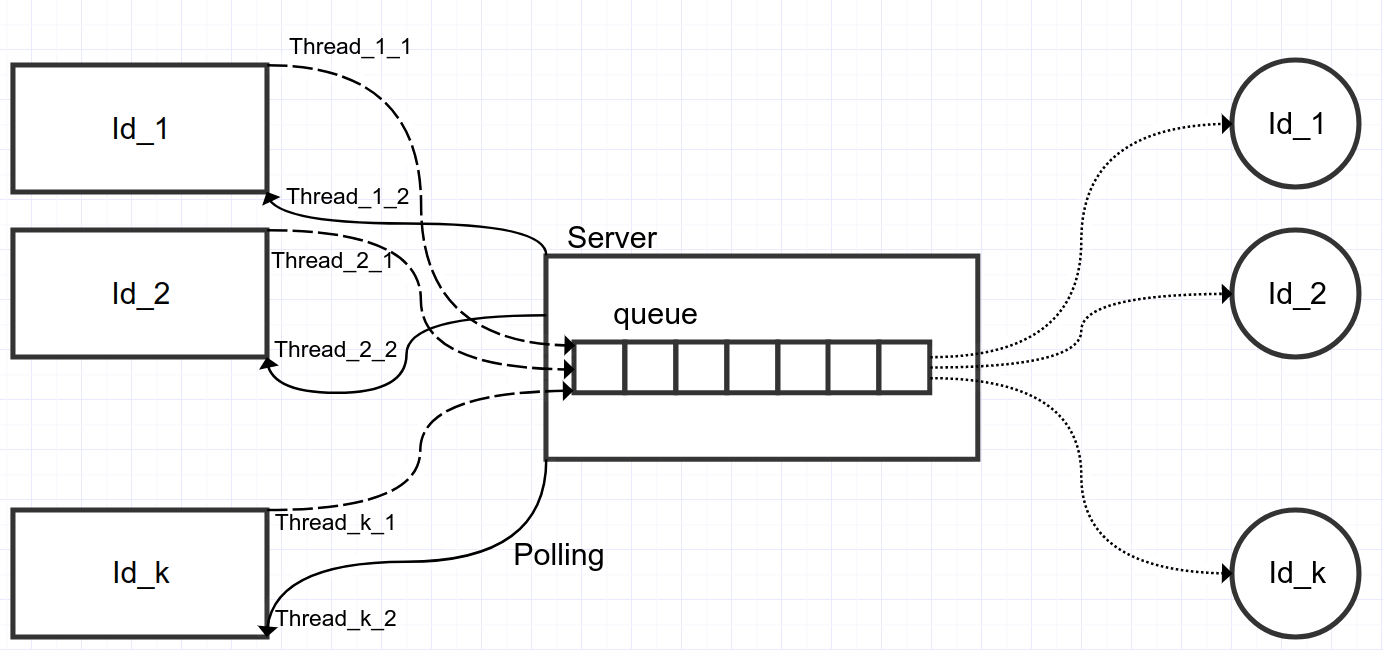
\includegraphics[width=0.85\textwidth]{diagram.png}
    \caption{Architecture of the simulated system}
    \label{fig:arch_diagram}
\end{figure}

\begin{figure}[H]
    \centering
    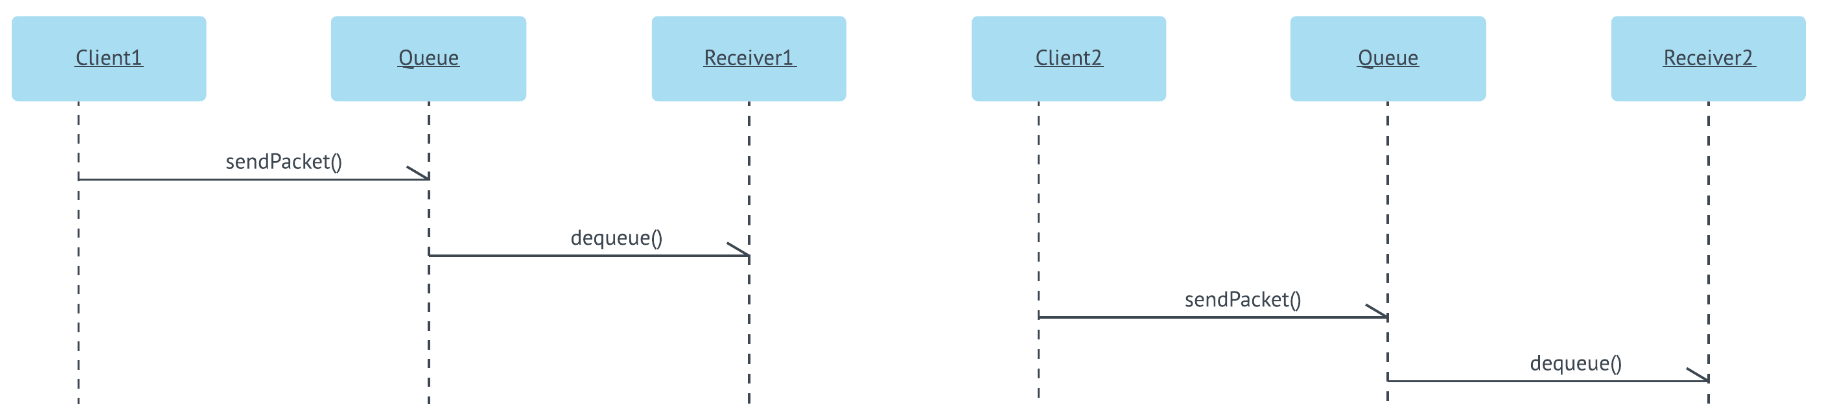
\includegraphics[width=0.95\textwidth]{UML_seq_diagram.png}
    \caption{UML sequence diagram}
    \label{fig:uml_diagram}
\end{figure}


\section{Implementation and execution}

The implementation was carried out by first coding the pure interrupt system. For this, each user thread sends $m$ packets in batches of $n$ packets each (these parameters are chosen by the user). These packets are sent to the queue where they are kept until there is an interruption, which in this case means that there are $50i$ items in the queue, with $i \in \mathbb{N}$. When the queue starts resending the packets, the senders may still send packets but they are lost because the queue is busy so it cannot attend these requests. After this, the polling round-robin system was implemented. As mentioned before, for each client there is a special user thread that is listening and waiting for the signal to start polling. The implementation can be run on any computer with the JVM and the Java compiler.

To compile the program with the \texttt{javac} compiler, the following command must be run:

\texttt{\$ javac UDPClient.java UserAPPS.java ServerQueue.java DevicesIO.java}

After this, three commands must be executed independently. The first command executes the file that contains the class that simulates the I/O devices called \texttt{DevicesIO}. For instance, to run the interrupt system, one has to execute:

\texttt{\$ java DevicesIO -c 50 -p 0 -n 100}

And to run the polling system with a quota of 10, one has to execute:

\texttt{\$ java DevicesIO -c 30 -p 10 -n 100}

Here we notice the \texttt{-c, -p, -n} parameters. These parameters must always be present and the order shall not be changed. The \texttt{n} parameter specifies how many packets will be sent, and the \texttt{c} parameter specifies the number of clients. The \texttt{p} parameter controls the quota of the queue. To use interrupts, the value of the parameter must be \texttt{0}.

After executing the \texttt{DevicesIO} file, one must execute the class that simulates the queue to receive and dispatch the packets. This is done with either of the following commands, the first one for interrupt system and the second one for the polling system:

\texttt{\$ java ServerQueue -c 50 -p 0 -n 100 > output.txt}

\texttt{\$ java ServerQueue -c 30 -p 10 -n 100 > output.txt}

To save the statistics that are generated, it is suggested to save the output to a file like done in the previous lines. This is done this way because in previous attempts, the delay from saving to disk created inconsistencies in the numbers.

Finally, to start the simulation, it is necessary to execute the class that takes care of sending the packets, this is done in the \texttt{UsedAPPS} file. For the interrupt system we run:

\texttt{java UserAPPS -c 50 -p 0 -n 100}

And for the polling system we run:

\texttt{java UserAPPS -c 30 -p 10 -n 100}

\section{Results}

In this section we display detailed results of the tests we made on our implementation. All results were run on a MacBook Pro (17-inch, late 2011) with macOS Sierra version 10.12.6, Intel Core i7 2.4 GHz, 4 hyperthreading cores and 8 GB of RAM.

We first compared the input packet rate versus the output packet rage for the interrupt-only system, and then for the hybrid system (interrupt and polling). This means, we measured how many packets per second were sent from all of the clients to the queue, and how many packets per second were sent from the queue to the receiving nodes. We tested different rates, and the results can be seen in figures \ref{fig:interrupt_rates} and \ref{fig:polling_rates}.

In each of the experiments, the number of total messages sent was chosen a priori in a fixed time, but as can be seen in the figures, the throughput did not vary much. And even more, there is not much difference between the interrupt system and the polling system. The outliers are probably caused by variation in the OS scheduler.

In figure \ref{fig:percentage_received}, we see the number of packages sent by all clients versus the percentage of packages received for each of the experiments and type of system. These plots show that there is no apparent pattern between the number of packages sent and the percentage of lost packages in transmission.

We believe that these results are due to the OS scheduler that efficiently handles the packets that are sent even when the queue size is really small, so we cannot stress the threads enough so that the results of the paper were successfully replicated with our implementation.

\begin{figure}[H]
    \centering
    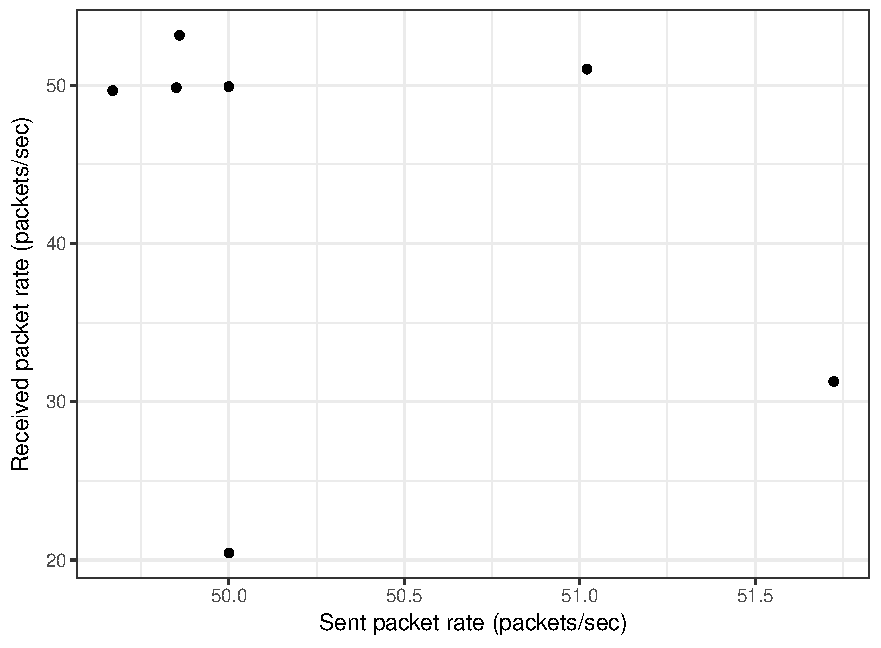
\includegraphics[width=0.75\textwidth]{interrupt_rates.pdf}
    \caption{Sent and received rates when a pure interrupt system is used}
    \label{fig:interrupt_rates}
\end{figure}


\begin{figure}[H]
    \centering
    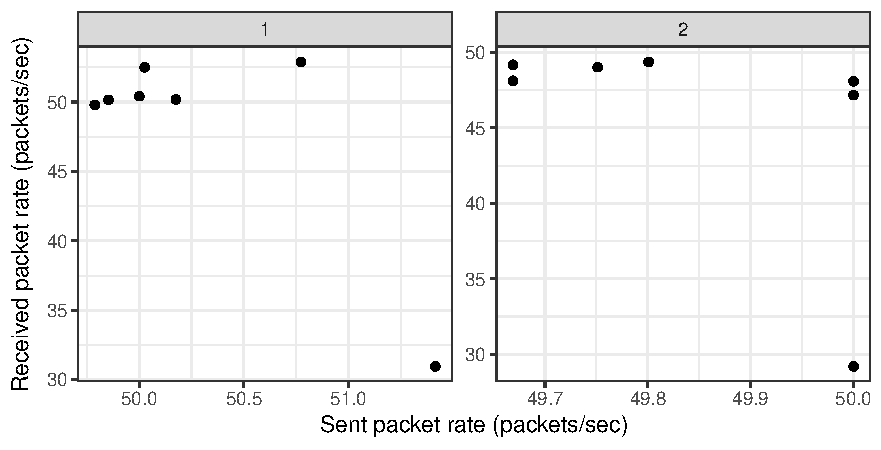
\includegraphics[width=0.75\textwidth]{polling_rates.pdf}
    \caption{Sent and received rates when the hybrid system is used (polling and interrupts)}
    \label{fig:polling_rates}
\end{figure}


\begin{figure}[H]
    \centering
    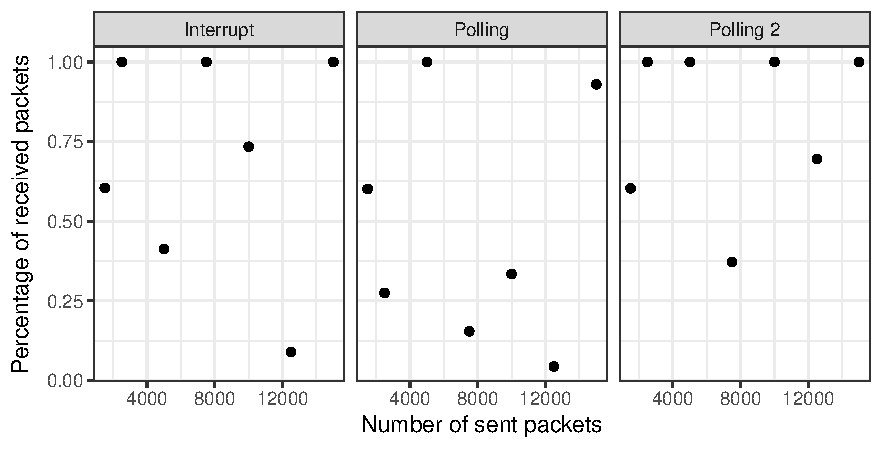
\includegraphics[width=0.75\textwidth]{number_packets_vs_percentage_received.pdf}
    \caption{Number of packets sent vs. percentage of packets received}
    \label{fig:percentage_received}
\end{figure}



\section{Conclusions}

In this work we implemented a program that intends to replicate the work done in \citetitle{mogul1997eliminating} \cite{mogul1997eliminating}. The theory in the paper was followed in the implementation, but nevertheless the results achieved are not aligned with the ones that are shown in the article, and we believe this is because our implementation is superseded by the more efficient OS scheduler, so the threads are not sufficiently stressed to cause a livelock in the computer. 

One of the things we learned in this project was that threads are hard to work with, and some unintuitive results can happen when working with them, things that would not happen when working with a sequential programming paradigm.

\printbibliography
%\nocite{*}


\end{document}
